% Template for PLoS
% Version 1.0 January 2009

\documentclass[10pt]{article}

% amsmath package, useful for mathematical formulas
\usepackage{amsmath}
% amssymb package, useful for mathematical symbols
\usepackage{amssymb}

% graphicx package, useful for including eps and pdf graphics
% include graphics with the command \includegraphics
\usepackage{graphicx}

% cite package, to clean up citations in the main text. Do not remove.
\usepackage{cite}

\usepackage{color} 
\usepackage[CaptionAfterwards]{fltpage}
\usepackage{floatrow}
% Use doublespacing - comment out for single spacing
%\usepackage{setspace} 
%\doublespacing


% Text layout
\topmargin 0.0cm
\oddsidemargin 0.5cm
\evensidemargin 0.5cm
\textwidth 16cm 
\textheight 21cm

% Bold the 'Figure #' in the caption and separate it with a period
% Captions will be left justified
\usepackage[labelfont=bf,labelsep=period,justification=raggedright]{caption}

% Use the PLoS provided bibtex style
\bibliographystyle{plos2009}

% Remove brackets from numbering in List of References
\makeatletter
\renewcommand{\@biblabel}[1]{\quad#1.}
\makeatother


% Leave date blank
\date{}

\pagestyle{myheadings}
%% ** EDIT HERE **


%% ** EDIT HERE **
%% PLEASE INCLUDE ALL MACROS BELOW

\newcommand{\Kcomment}[1]{{\color{blue}{[KJ: #1]}}}
\newcommand{\Acomment}[1]{{\color{red}{[AE: #1]}}}

\DeclareMathOperator{\Tr}{tr}
\newcommand{\sq}[1]{\lq#1\rq}
\newcommand{\mcond}{\,\middle\vert\,}
\newcommand{\cond}{\,\vert\,}
\newcommand{\figref}[2]{Fig.\;\ref{fig:#1}\,#2}
\newcommand{\loss}[1]{\mathcal L\left(#1\right)} 
\newcommand{\eloss}[1]{\mathcal L_0\left(#1\right)}
\newcommand{\T}{{\sf T}}
\newcommand{\E}[2][]{\mathbb E_{#1}\left[ #2\right]}    % expected value
\newcommand{\TODO}[1]{\emph{\small\color{blue}$\langle\langle$#1$\rangle\rangle$}}
\newcommand*\dif{\mathop{}\,d}
\DeclareMathOperator*{\argmin}{arg\,min}
\DeclareMathOperator{\rank}{rank}

%% END MACROS SECTION

\begin{document}
% Title must be 150 characters or less
\begin{flushleft}
{\Large
Partial neural correlations suggest detailed interactions in cortical circuits
}
% Insert Author names, affiliations and corresponding author email.
\\
Dimitri Yatsenko,$^{1,\ast}$, 
Kre\v{s}imir Josi\'{c}$^{2}$,
Alexander S.~Ecker$^{1,3,4}$,
Emmanouil Froudarakis$^{1}$,
R.~James Cotton$^{1}$,
Andreas S.~Tolias$^{1,5}$
\\
\bf{1} Department of Neuroscience, Baylor College of Medicine, Houston, TX, USA
\\
\bf{2} Department of Mathematics and Department of Biology and Biochemistry, University of Houston, Houston, TX, USA
\\
\bf{3}  Werner Reichardt Center for Integrative Neuroscience and Institute for Theoretical Physics, University of T\"ubingen, Germany
\\
\bf{4} Bernstein Center for Computational Neuroscience, T\"ubingen, Germany
\\
\bf{5} Department of Computational and Applied Mathematics, Rice University, Houston, TX, USA

$\ast$ E-mail: yatsenko@cns.bcm.edu
\end{flushleft}

\section*{Abstract}
% Please keep the abstract between 250 and 300 words
Ambitious projects aim to record the activity of ever larger and denser subsets of neurons \emph{in vivo}.  Correlations in neural activity measured in such recordings can reveal important aspects of the functional organization of neural circuits.  However, estimating and interpreting large correlation matrices obtained from finite recordings is challenging.  Estimation can be improved by regularization, \emph{i.e.}\;by imposing a structure on the estimate.  The amount of improvement depends on how closely the assumed structure represents dependencies in the data. Therefore, the selection of the most efficient correlation matrix estimator for a given neural circuit must be determined empirically.  Furthermore, the identity and structure of the most efficient estimator informs about the types of dominant dependencies governing the system.

We sought the most statistically efficient estimators of neural correlation matrices in recordings from large, dense groups of cortical neurons.  Using fast 3D random-access laser scanning microscopy of calcium signals, we recorded the activity of nearly every neuron in volumes of about 200 $\mu$m wide and 100 $\mu$m deep (150--350 cells) in mouse visual cortex.  We hypothesized that in these dense recordings, the correlation matrix should be most efficiently represented as the combination of a sparse matrix of pairwise partial correlations representing local interactions and a low-rank component representing common fluctuations and external inputs.  Indeed, in cross-validation tests, the covariance matrix estimator with such structure consistently outperformed other regularized estimators. The connectivity patterns inferred from the sparse component of the estimate manifested a strong relationship to the geometrical arrangement and orientation tuning properties of cells: the density of positive \sq{excitatory} connections decreased rapidly with geometric distance and the difference in orientation preference whereas the negative \sq{inhibitory} connections were less selective.  Because of its superior performance, this estimator likely provides a more physiologically relevant representation of the functional connectivity in dense recordings than sample correlations.

\section*{Author Summary}
% Please keep the Author Summary between 150 and 200 words
% Use first person. PLoS ONE authors please skip this step. 
% Author Summary not valid for PLoS ONE submissions.   
Correlations in the activity of neural populations have proven useful as descriptions of the functional connectivity in the embedding circuit.  Correlations may arise from various underlying processes that reflect differently on the structure of the correlation matrix:  Common network fluctuations or external inputs are well approximated by low-rank representations whereas linear effects between specific pairs of neurons are well approximated by fitting their pairwise partial correlations.  What kinds of correlation effects dominate the population activity in cortical microcircuits? To answer this question, we imposed various correlation structures on empirical estimates of neural correlation matrices and evaluated which of them produced greatest estimation improvement.  In fast 3D two-photon imaging of calcium signals of large and dense groups of neurons in mouse visual cortex, the greatest improvement was produced by decomposing the correlation matrix as a sparse network of partial correlations and a low-rank component.  Since it leads to the best estimates, we propose that this structure provides a better picture of the functional connectivity than that obtained from sample correlations. As an application of this approach, we analyzed how the inferred connectivity related to distances between cells and to differences in their preferred orientations and found basic resemblance to results from studies of synaptic connectivity.
\section*{Introduction}
\paragraph{Neural correlations}
Pearson correlations between the spiking activity of pairs of neurons, or simply \emph{neural correlations}, are among the most familiar descriptive statistics of neural population activity \cite{Averbeck:2006, Zohary:1994, Kohn:2005, Bair:2001, Ecker:2010}.  For example, \emph{noise correlations}, \emph{i.e.}\;the correlations of trial-to-trial response variability between pairs of neurons, have a profound impact on stimulus coding \cite{Zohary:1994, Abbott:1999, Sompolinsky:2001, Nirenberg:2003, Averbeck:2006, Josic:2009, Berens:2011, Ecker:2011}. In addition, noise correlations and correlations in spontaneous activity have been hypothesized to reflect key features of the functional connectivity in neural circuits \cite{Gerstein:1964}.  This interpretation is supported by a series of discoveries of nontrivial relationships between neural correlations and other aspects of circuit organization such as the physical distances between neurons \cite{Smith:2008, Denman:2013}, their synaptic connectivity \cite{Ko:2011},  stimulus response similarity \cite{Bair:2001, Arieli:1995, Chiu:2002, Kenet:2003, Kohn:2005, Cohen:2008, Cohen:2009, Ecker:2010,Ko:2011, Smith:2013b}, cell types \cite{Hofer:2011}, cortical layer specificity \cite{Hansen:2012, Smith:2013}, progressive changes in development and in learning \cite{Golshani:2009, Gu:2011}, changes due to sensory stimulation and global brain states \cite{Goard:2009, Kohn:2009, Ecker:2010, Renart:2010} among others.

However, neural correlations do not submit to ready or unambiguous mechanistic interpretation.  Theoretical studies and simulations have shown that neural correlations on various temporal scales may arise from combinations of multiple mechanisms including direct synaptic interactions, common inputs or correlated inputs, chains of multiple synaptic connections, oscillations, top-down modulation, and background network fluctuations \cite{Perkel:1967, Moore:1970, Shadlen:1998, Salinas:2001, Ostojic:2009, Rosenbaum:2011}. 

\paragraph{Structure  of correlation matrices}
Modern multineuronal recordings allow measuring entire correlation matrices from increasingly large and dense populations of highly interconnected neurons. Multivariate analysis techniques based on large correlation matrices provide information that could not be extracted from an equivalent number of isolated measurements of pairwise correlations.  For example, when the correlation matrix is approximated in a form with a reduced number of variables, this \emph{reduced representation} can isolate an important aspect of the functional connectivity in neural circuits and possibly point to underlying physiological mechanisms and computational principles. 

One reduced representation of the correlation matrix is its low-rank approximation.  Low-rank approximations are particularly suitable for capturing common fluctuations and common external inputs and can be extracted using principal component analysis, independent component analysis, factor analysis, or  \cite{Chapin:1999, Peyrache:2010, Lopes:2011, Lopes:2013}.

Another reduced representation of the correlation matrix can be obtained by \emph{covariance selection}, \emph{i.e.}\;by selecting a subset of the pairwise \emph{partial correlations} that are sufficient to reproduce the entire correlation matrix \cite{Dempster:1972, Friedman:2008}. The partial correlation between a pair of neurons is a measure of their linear association after the effects of the rest of the network have been taken into account \cite{Anderson:2003}. Partial correlations are particularly meaningful when all effects between the variables are nearly linear and a large fraction of the variables are observed; in this case, partial correlations approximate conditional dependency.  A lack of conditional dependency between two neurons suggests a lack of direct interaction between them. Networks of partial correlations (sometimes called \emph{association networks}) have been used to infer gene interaction networks \cite{Schafer:2005, Peng:2009} and interactions between brain regions in brain imaging studies \cite{Varoquaux:2012, Ryali:2012}. 

\paragraph{Improving estimation through regularization}
Imposing a structure on an estimate of the covariance matrix can improve its estimation performance.  

Estimation of covariance matrices from large populations presents a number of numerical challenges:  The amount of recorded data grows only linearly with population size whereas the number of estimated coefficients increases quadratically.  This mismatch leads to an increase in spurious correlations, overestimation of common activity (\emph{i.e.}\;overestimation of large eigenvalues) \cite{Ledoit:2004}, and poorly conditioned partial correlations \cite{Schafer:2005}.  

In neuroscience studies, the true correlation matrix is usually estimated by the \emph{sample correlation matrix}, which is rarely distinguished from the true correlation matrix.  The sample correlation matrix is unbiased but, because it has many free parameters, it is highly sensitive to sampling noise. As a result, on average, the sample correlation matrix is far from the true correlation matrix.  In contrast, reduced estimates are typically less susceptible to sampling noise although can introduce their respective biases.  

In statistics, the technique of deliberately imposing a structure on an estimate in order to improve its performance is known as \emph{regularization} \cite{Schafer:2005, Bickel:2006}.    To \sq{impose structure} on an estimate means to bias (\sq{shrink}) it toward a reduced representation known as the shrinkage target.  The selection of the optimal target estimate and the optimal amount of shrinkage can be deduced from the training data either analytically or by cross-validation.  Some regularization schemes only perform target selection (\emph{dimensionality reduction, variable selection, or feature selection}) and replace the estimate completely. Others only perform shrinkage toward a single target estimate (\emph{shrinkage estimators}).  Yet others can do both target selection and shrinkage toward the target.

Although regularized covariance matrix estimates have become commonplace in other fields such as finance \cite{Ledoit:2003}, functional genomics \cite{Schafer:2005}, and brain imaging \cite{Ryali:2012}, surprisingly little work has been done to identity optimal regularization of neural correlation matrices.  
\paragraph{Illustration of estimation of a neural correlation matrix}
To illustrate the challenges and techniques of estimation of the correlation matrix from a finite sample, we consider a regularization scheme based on \emph{covariance selection} (Figure \ref{fig:01}) \cite{Dempster:1972, Friedman:2008}. Here the estimate is produced by fitting only an optimal subset of the coefficients of the precision matrix (inverse of the covariance matrix) while setting the rest to zero.  Zeros in the off-diagonal elements of the precision matrix indicate zero partial correlations between the corresponding pair of neurons.   Therefore, covariance selection amounts to finding an approximation of the covariance matrix that maximizes the number of neuron pairs that are linearly independent of each other when conditioned on the activity of all the other observed cells. 

We estimated the covariance matrix of somatic calcium signals of a group of 298 neurons in mouse visual cortex using both the sample covariance matrix (\figref{01}{A, B}) and covariance selection (\figref{01}{C}). Due to the low-pass filtration effect of calcium dye kinetics, correlations in unprocessed calcium signals are higher than typical firing rate correlations on shorter temporal scales. The close similarity of the two estimates of the correlation matrix (\figref{01}{B and C}) belies the utterly different partial correlation structure (\figref{01}{D and E}): The regularized estimate is produced from the same data by setting to zero 31,501 (71.2\%) of the off-diagonal coefficients of the precision matrix and fitting the remaining 12,752 coefficients. 

Estimation by covariance selection is attractive for several reasons: First, with fewer free parameters it is less susceptible to sampling noise, yielding estimates that are, on average, closer to the truth. Additionally, if we assume that partial correlations do indeed reflect elements of the functional connectivity in the circuit, the second estimate also appears more plausible: in neural circuits, each neuron only interacts with a fraction of the entire population. 

\begin{figure}[!ht]    \floatbox[{\capbeside\thisfloatsetup{capbesideposition={right,center},capbesidewidth=8.3cm}}]{figure}[\FBwidth]
    {\caption{{\bf Illustration of regularized estimation of partial correlations.}
        {\bf A}. The sample correlation matrix of unprocessed somatic calcium signals from a population of cells in mouse visual cortex.
        The outlined square fragment is magnified in {\bf B}.
        {\bf C}. The same fragment of another estimate of the correlation matrix regularized to yield sparse partial correlations.
        Corresponding fragments of partial correlations matrices of the unregularized and regularized estimated are shown in {\bf D} and {\bf E}, respectively.
    }
    \label{fig:01}}
    {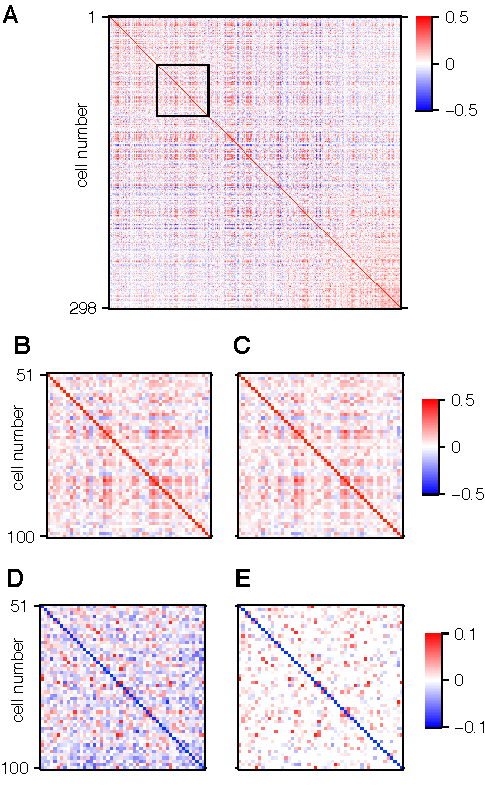
\includegraphics[width=8.3cm]{./figures/Figure01.pdf}}
\end{figure}
\paragraph{Conceptual questions and basic approach}
What structures of correlation matrices best describe the multineuronal activity in specific circuits and in specific brain states?  More specifically, are correlations in the visual cortex during visual stimulation best explained by common fluctuations or by local interactions within the recorded microcircuit? 

To address these questions, we evaluated five covariance matrix estimators based on different assumptions about the underlying correlation structure:
\begin{description}
\item[$C_{\sf 0}$] -- sample covariance matrix, the unbiased, unregularized estimator.
\item[$C_{\sf diag}$] -- linear shrinkage toward a diagonal covariance matrix. 
\item[$C_{\sf factor}$] -- linear shrinkage toward a low-rank matrix produced by factor analysis.
\item[$C_{\sf sparse}$] --  sparse partial correlations, \emph{i.e.}\;covariance selection.
\item[$C_{\sf sparse+latent}$] -- sparse partial correlations between the recorded neurons combined with partial correlations with several inferred latent units.
\end{description} 

First, we demonstrated that, in simulations with known true correlation structures, estimators that imposed a matching structure were generally more efficient than the other estimators.  The estimators� relative performance was evaluated by cross-validation.   The logic of this study relies on the converse of this relationship: the covariance matrix estimator that is found to be most efficient on empirical data is proposed to provide a better picture of the correlation structure than other estimators.  Caveats for this type of inference are reviewed in the Discussion.

Therefore, we performed a cross-validated evaluation to establish which of the four regularized estimators was most efficient for the population activity of dense groups of neurons in mouse primary visual cortex recorded with fast 3D random-access two-photon imaging of calcium signals. We found that $C_{\sf sparse+latent}$ consistently outperformed the other estimators.  This estimator produced a sparse network of partial correlations between the observed neurons combined with correlations between several inferred latent units.  We examined the structure of the sparse partial correlations inferred by the estimate with respect to the neurons� geometrical positions and preferred orientations and found that stronger dependencies than those of sample correlations. In Discussion, we outline possible approaches to further corroborate the relationship between the structure of the functional connectivity revealed by such methods to the anatomical organization of the circuit.

\section*{Results}
% Results and Discussion can be combined.
\paragraph{Covariance estimation}
The icovariance matrix defined as
\begin{equation}\label{eq:true-covariance}
    \Sigma = \E{(x-\mu)(x-\mu)^\T},\quad \mu = \E{x}
\end{equation}
where $\E{\cdot}$ denotes expectation; $x$ is the $p\times 1$ vector of real-valued instantaneous firing rates in bins of duration $\Delta t$; and $\mu$ is the vector of mean firing rates. In the case of noise correlations, $\mu$ depends on the stimulus condition.  Usually, neural covariance matrices have been estimated as the \emph{sample covariance matrix} $C_{\sf 0}$ calculated from the empirical sample of observations $x(t),\; t=n(1,\ldots,n)$ as
\begin{equation}
    C_{\sf 0} = \frac 1 \nu \sum\limits_{t=1}^n (x(t)-\bar x)(x(t)-\bar x)^\T,\quad \bar x= \frac 1 n \sum\limits_{t=1}^n x(t)
\end{equation}
where $\nu$ is the number of degrees of freedom per neuron in the sample ($\nu=n-1$ if observations are independent). In this study, we estimate the true mean, $\mu$, using the sample mean $\bar x$, but seek a better estimate of the covariance matrix than $C_{\sf 0}$.  In the case of noise correlations, the true mean $\mu$ and the sample mean $\bar x$ are conditioned on the stimulus.

Given a covariance matrix estimate $C$ (not necessarily the sample covariance $C_{\sf 0}$), the correlation matrix $R$ is calculated by normalizing $C$ by its diagonal (variance estimates):
\begin{equation}\label{eq:precision}
    R = \left(I\circ C\right)^{-\frac 1 2} C \left(I\circ C\right)^{-\frac 1 2}
\end{equation}
Similarly, the matrix of partial correlations $P$ is computed by normalizing the the negative \emph{precision matrix} $C^{-1}$ (inverse of the covariance matrix):
\begin{equation}\label{eq:partial}
    P = -\left(I\circ C^{-1}\right)^{-\frac 1 2} C^{-1} \left(I\circ C^{-1}\right)^{-\frac 1 2}
\end{equation}
Here $\circ$ denotes entrywise matrix product (Hadamard product) and $I$ is the $p\times p$ identity matrix. Clearly, off-diagonal zeros in the precision matrix correspond to zero partial correlations. 

We considered four regularized estimators based on distinct families of low-dimensional target estimates: $C_{\sf diag}$, $C_{\sf factor}$, $C_{\sf sparse}$, and $C_{\sf sparse+latent}$. In probabilistic models with exclusively linear dependencies, their targets estimates can be described by distinct families of graphical models (\figref{02}{row 1}).  

\begin{FPfigure}
    \begin{center}
        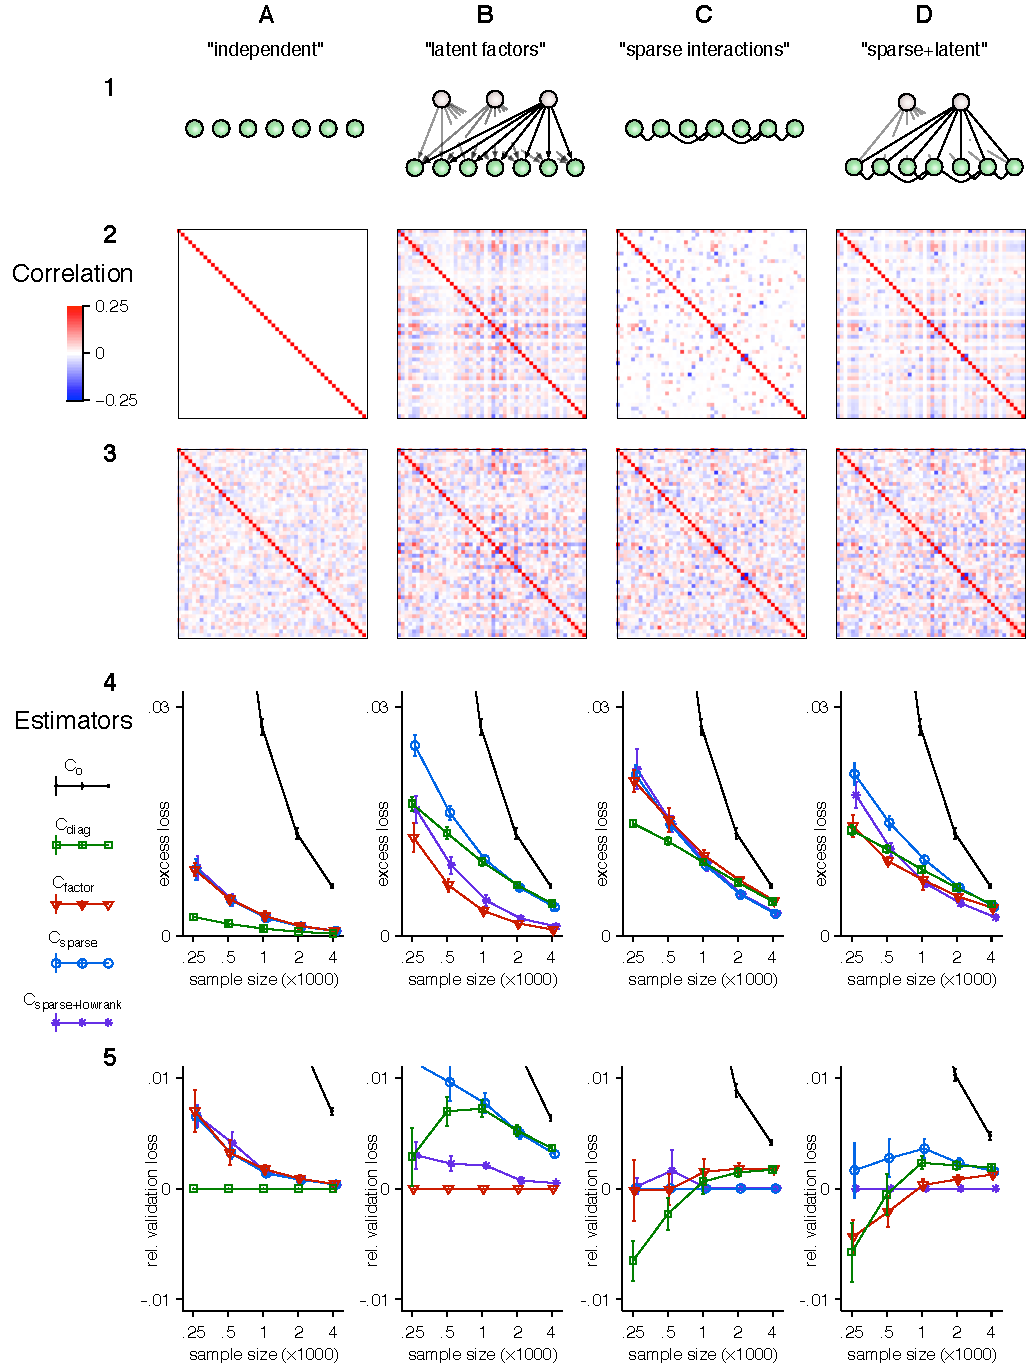
\includegraphics{./figures/Figure02.pdf}
    \end{center}
    \caption{{\bf Estimators whose low-dimensional regularization targets can represent the structure of the true covariance matrix outperform other estimators.}
        {\bf Row 1.} Graphical representations of four types of low-dimensional structures of interactions between observed neurons (green spheres) and latent units (light-shaded spheres).
        In the \sq{independent model} ({\bf A}), observed neurons exert no linear effects on one another neither directly nor through interactions with common latent units. 
        In \sq{latent factors} ({\bf B}), the correlated activity of observed cells is driven by several latent units. 
        In \sq{sparse interactions} ({\bf C}), the correlation matrix is defined by a set of linear interactions between observed neurons. 
        In \sq{sparse+latent} ({\bf D}), correlations arise through direct linear interactions in a sparse subset of observed neurons and through interactions with common latent units. 
        {\bf Row 2.} Examples of $50\times 50$ correlation matrices corresponding to each type of low-dimensional structure. 
        The factor model ({\bf B}) has three latent units. 
        The partial correlation matrix of the sparse model ({\bf C}) is 73\% sparse.
        The \sq{sparse+latent} matrix has one latent unit and its direct interactions are 78\% sparse.
        {\bf Row 3.} Examples of sample correlation matrices calculated from samples of 1000 observations taken from simulated random processes with corresponding correlation matrices from row 2.
        {\bf Row 4.} Mean \emph{excess loss} (Eq.~\ref{eq:excess-loss}) attained by each of the five estimators as a function of sample size. The error bars indicate the standard error of the mean based on 30 samples.
        {\bf Row 5.} Mean \emph{cross-validation loss} (Eq.~\ref{eq:rel-cv-loss}) of covariance estimators with respect to the matching estimator. The values are relative to the validation loss of the estimator that matches the low-dimensional structure of the true covariance matrix. Error bars indicate the standard error of the mean based on 30 samples.
    }
    \label{fig:02}
\end{FPfigure} 

For estimator $C_{\sf diag}$, the target estimate is the diagonal matrix $D$ whose diagonal contains  variance estimates. Regularization is achieved by linear \emph{shrinkage} of the unbiased estimate $C_{\sf 0}$ toward $D$ controlled by the scalar \emph{shrinkage intensity} parameter $\lambda \in [0, 1]$:
\begin{equation}\label{eq:c-diag}
C_{\sf diag} = (1-\lambda) C_{\sf 0} + \lambda D
\end{equation}
The structure of target $D$ favors the absence of linear associations between the activity of observed neurons (\figref{02}{A}).  If sample correlations arise from spurious or contingent effects, $C_{\sf diag}$ should outperform the other estimators. 

The target of estimator $C_{\sf factor}$ is the factor model $L + \Psi$, where $L$ is the $p\times p$ positive definite matrix of rank $d$, and $\Psi$ is the diagonal matrix of independent variances.  The estimator, 
\begin{equation}\label{eq:c-factor}
C_{\sf factor} = (1-\lambda) C_{\sf 0} + \lambda (L + \Psi),
\end{equation}
has two hyperparameters: the number of factors $d$ and shrinkage intensity $\lambda$. The target estimate $L + \Psi$ has the structure that arises when correlated fluctuations in population activity are linearly driven by a number of latent factors that affect many cells while direct interactions between cells are insignificant (\figref{02}{B}).   

Estimator $C_{\sf sparse}$ is based on the assumption that correlations result from direct linear associations between pairs of observed neurons and that only a fraction of neuron pairs interact (\figref{02}{C}).  This assumption is enforced by fitting only a subset of the off-diagonal elements of the precision matrix while setting the rest to zero. The estimator takes the form
\begin{equation}\label{eq:c-sparse}
C_{\sf sparse} = S^{-1},
\end{equation}
where $S$ is a sparse matrix with a large fraction of zeros in its off-diagonal.  The estimate has one hyperparameter that determines the sparsity (fraction of off-diagonal zeros) of $S$.

Estimator $C_{\sf sparse+latent}$ allow the assumptions of both $C_{\sf factor}$ and $C_{\sf sparse}$.  Its correlation structure can be explained by linear effects exerted between some pairs of observed neurons and several latent units (\figref{02}{D}). The estimator has the form \cite{Chandrasekaran:2010,Ma:2013}:
\begin{equation}\label{eq:c-sl}
C_{\sf sparse+latent} = (S - L)^{-1}
\end{equation}
where, as above, $S$ is a sparse matrix and $L$ is a $p\times p$ matrix of rank $d$. The estimator has two hyperparameters: one to regulate the number of latent units, the other to regulate the sparsity of matrix $S$.

\paragraph{Simulation}
To illustrate the performance of the four regularized estimators, we constructed four model populations of $p=50$~neurons each with each matching the correlation structures of a different target estimate (\figref{02}{\,Row 2}).  Sample correlation matrices calculated from samples of size $n=1000$ contain substantial sampling noise (\figref{02}{\,Row 3}) that makes the correlation structure less obvious.

An evaluation of the performance of a covariance matrix estimator $C$ requires a real-valued \emph{loss function} $\loss{C,\Sigma}$. The loss loss function quantifies the deviation of the estimate $C$ from truth $\Sigma$ and attains its minimum when $C=\Sigma$.

In this study, we adopted the \emph{normal loss} defined as
\begin{equation}\label{eq:loss}
    \loss{C,\Sigma} = \frac 1 p\left[\ln \det C + \Tr(C^{-1}\Sigma)\right]
\end{equation}

This loss function relates to the multivariate normal log-likelihood function $L(\Sigma|C_{\sf 0})$ through the following expression:
\begin{equation}
    L(\Sigma|C_{\sf 0}) = -\frac p 2 \ln(2\pi) -\frac p 2 \loss{\Sigma,C_{\sf 0}}
\end{equation}
Although the two functions appear similar in form, they differ conceptually: The log-likelihood is a function of the parameter $\Sigma$ given the sample covariance matrix $C_{\sf 0}$ whereas the loss function expresses the distance from an arbitrary estimate $C$ to the given truth $\Sigma$.

The normalization by $\frac 1 p$ is not standard but serves to make the values of the loss functions comparable across different population sizes. 

The choice of loss function is motivated by mathematical convenience. We expect that the main conclusions of our study will not change qualitatively with other well behaved loss functions, such as the Frobenius norm of the difference $\|C-\Sigma\|_F$ \cite{Ledoit:2004,Schafer:2005}, Stein's entropy loss, or quadratic loss \cite{James:1961,Fan:2008}.  

We define the \emph{excess loss} as
\begin{equation}\label{eq:excess-loss}
    \eloss{C,\Sigma} = \loss{C,\Sigma}-\loss{\Sigma,\Sigma},
\end{equation}
which assumes zero at its minimum. 

We computed the excess losses for 30 samples for each sample size $n=250$, 500, 10000, 2000, and 4000 for each of the five estimators and for each ground truth (\figref{02}{\,row 5}). For each estimator, hyperparameters were estimated by nested cross-validation (See Methods.).  As expected, estimators whose structure matched that of the true model typically outperformed the other estimators. There were two exceptions: First, for some smaller samples, the data were insufficient to reveal the true correlation structure and the estimators with the simpler structure, $C_{\sf diag}$ and $C_{\sf factor}$ outperformed the estimators with matching structure (\figref{02}{\,columns C and D, rows 5 and 6}).  Second, $C_{\sf sparse+latent}$ often performed equally well to the sparse estimator even when the ground truth did not have any latent units.  In these cases, it inferred the right number of latent units, zero, and estimated optimally.

When the ground truth, $\Sigma$, is not accessible, loss can be estimated solely from the data through \emph{validation}.  In validation, an additional independent \emph{testing sample} is used to compute a sample covariance estimate $C_{\sf 0}^\prime$.  Then \emph{validation loss} $\loss{C,C_{\sf 0}^\prime}$ can be used as an estimate of loss $\loss{C,\Sigma}$.  Thus, estimators resulting in consistently lower validation loss can be inferred to produce estimates that are closer to truth than estimators with higher validation loss.

The negative log-likelihood loss (Eq.~{\ref{eq:loss}) is particularly convenient because it is additive in its second argument in the sense that 
 \begin{equation*}\label{eq:additivity}
 \loss{C,z_1} + \loss{C,z_2} \equiv \loss{C,z_1+z_2}
 \end{equation*}

Then the cross-validation loss is in fact an unbiased estimate of loss.
\begin{equation*}
    \E[C_{\sf 0}^\prime]{\loss{C,C_{\sf 0}^\prime}}=\loss{C,\E[C_{\sf 0}^\prime]{C_{\sf 0}^\prime}}=\loss{C,\Sigma}
\end{equation*}

The property of additivity does not hold for other popular loss functions such as Stein's entropy loss or various quadratic losses.  With non-additive loss functions, validation loss is a biased estimate of loss, but it is still generally appropriate to be used in lieu of loss.

With empirical data, acquiring a separate testing sample is not practical. Instead, $K$-fold cross-validation is used: The sample is divided into $K$ subsets of approximately equal size ($K=10$ in this study).  Then each subset is used as the validation sample with the other $K-1$ serving as the training sample. The validation losses from each of such \sq{folds} are averaged to produce the \emph{cross-validation loss} or \emph{CV-loss} for short.  Let $C_{\sf 0}^{\{k\}}$ denote the sample covariance matrix computed from the $k^{th}$ subset and $C^{\{\setminus k\}}$ denote the results of estimator $C$ trained on the remaining $K-1$ subsets. Then cross-validation loss for estimator $C$ is
\begin{equation}\label{eq:cv-loss}
    \ell_C=\frac 1 K \sum\limits_{k=1}^K \loss{C^{\{\setminus k\}},C_{\sf 0}^{\{k\}}}
\end{equation}
In this formulation, $\ell_C$ can be recognized as the cross-validated Gaussian log-likelihood (up to a constant offset and multiplier). However, the present framework is more general, allowing for other loss functions to be used.

Since we only need to compare estimators to each other, we are only interested in the \emph{relative} CV-loss of estimator $C$ with respect to reference estimator $C_{\sf ref}$:
\begin{equation}\label{eq:rel-cv-loss}
    \Delta\ell_{C,C_{\sf ref}} = \ell_{C}-\ell_{C_{\sf ref}}
\end{equation}

In simulation, CV-loss accurately reproduced the differences between the estimators' excess losses, although with greater variability (\figref{02}{Row 6}). For each kind of ground truth (Row 2), relative CV-losses were computed with respect to the estimator whose regularization target matched the structure of the respective ground truth. 

These simulations demonstrated that, with sufficiently large sample sizes, the most efficient among several regularized estimators could be used to infer the most likely type of correlation structure present in the data.

\paragraph{Covariance estimation in neural data}
We recorded calcium activity in dense populations of neurons in the supragranular layers in primary visual cortex of anesthetized mice using fast random-access 3D scanning two-photon microscopy \cite{Reddy:2005, Katona:2012, Cotton:2013}. We presented 300 repetitions of full-field drifting gratings with two directions of motion or 150 repetitions with five directions (\figref{03}{A}) on one side of the visual field of anesthetized mice. Groups of cells loaded with a calcium-sensitive fluorescent dye were imaged and localized in 3D space (\figref{03}{B and E}) in the visual cortex on the contralateral side to the stimulus. Using acousto-optic deflectors (AOD) to steer the laser in 3D, we recorded the somatic calcium activity from the located cells with concurrent motion detection \cite{Cotton:2013}.  This technique allowed fast sampling (100--150 Hz) from large numbers (150--350) of cells in a small volume of cortical tissue ($200\times200\times100$ $\mu$m$^3$) in layers 2/3 and 4 (\figref{03}{C}). After downsampling the signal to 20 Hz, relative firing rates were inferred using sparse nonnegative deconvolution \cite{Vogelstein:2010} (\figref{03}{C and D}). Only cells that produced detectable calcium activity were included in the analysis (See Methods). The average stimulus response was subtracted from each trial; the remaining signals were further downsampled into 150 ms bins to compute the noise correlation matrix (\figref{03}{F and G}). The durations of recordings dedicated to estimating the noise correlations ranged between 15--20 minutes.  Besides the high-repetition stimulus protocol used to estimate noise correlations, an orientation tuning stimulus protocol was used to map the orientation tuning of each cell (\figref{03}{E}). Overall, 31 imaged sites from 24 animals were included in the study.

\begin{figure}    \floatbox[{\capbeside\thisfloatsetup{capbesideposition={right,center},capbesidewidth=8.3cm}}]{figure}[\FBwidth]
    {\caption{{\bf Acquisition of neural signals for the estimation of noise correlations.}
    Visual stimuli comprising full-field drifting gratings interleaved with blank screens ({\bf A}) were presented to anesthetized mice while two-photon recordings of somatic calcium signals were collected using fast 3D random-access microscopy ({\bf B}). The visual stimulus included an initial period with 16 directions of motion for orientation tuning followed by a longer (15--20 min) period of stimulation with only 2 or 5 directions of motion for the computation of the noise correlation matrix. 
    {\bf C.} Representative calcium signals from eight cells out of 298 cells downsampled to 20 Hz. The inferred firing rate binned in 150 ms intervals are indicated by red ticks below each trace.
    {\bf D.} The raster plot of the inferred firing rates, binned in 150 ms intervals, from the entire population from the first (left) and last (right) minute of the entire recording.  The traces from {\bf C} are highlighted in red.
    {\bf E.} The spatial arrangement and orientation tuning of the 298 cells from the imaged site.
    {\bf F.} The noise correlation matrix of the activity of the neural population. 
    {\bf G.} Histogram of noise correlation coefficients. The red line indicates the mean.
} \label{fig:03}}
    {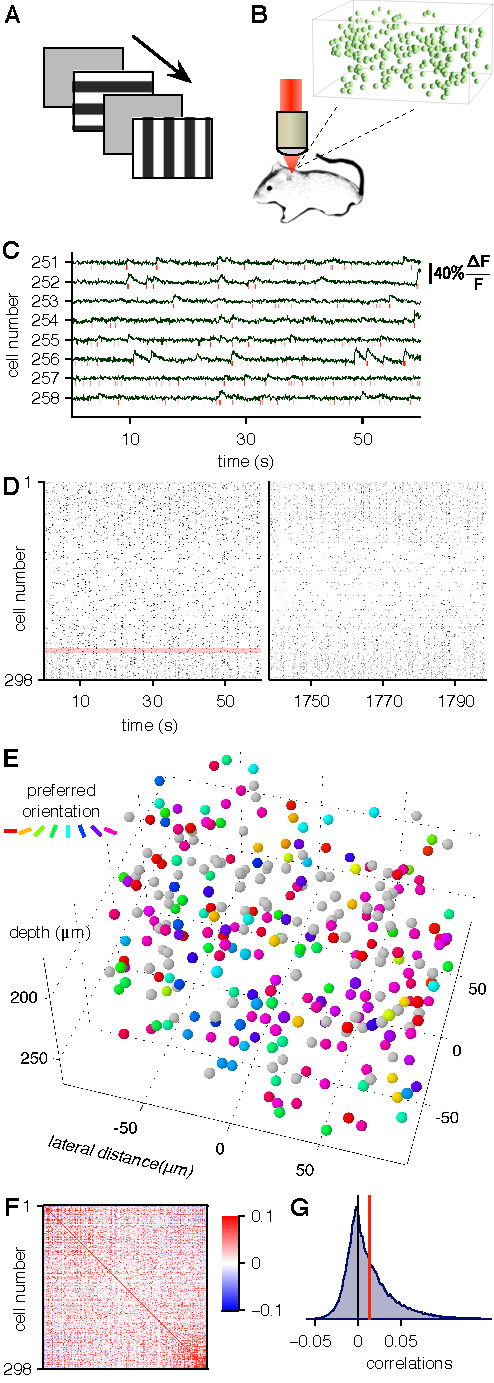
\includegraphics[width=8.3cm]{figures/Figure03.pdf}}
\end{figure}

In these highly localized populations both direct interactions between cells and common diffuse inputs likely contribute to overall population co-variability.  We therefore hypothesized that regularized estimates capturing a sparse partial correlation structure, and/or interactions with latent units would be the most efficient. At the same time, average correlations were relatively small (\figref{03}{G}), giving a potential advantage to estimates biased toward independence (\emph{e.g.}\;$C_{\sf diag}$). Finally, correlation structure could possibly be best explained by common fluctuations across the entire population, to the advantage of estimates biased toward low-rank correlation structure (\emph{e.g.}\;$C_{\sf factor}$, $C_{\sf sparse+latent}$). Thus it was \emph{a priori} unclear which estimator would perform best.

We found that estimator $C_{\sf sparse+latent}$ was the most efficient (Fig.~\ref{fig:04}). The median relative CV-validation loss (Eq.~\ref{eq:rel-cv-loss}) of each of the estimates $C_{\sf 0}$, $C_{\sf diag}$, $C_{\sf factor}$, and $C_{\sf sparse}$ with respect to $C_{\sf sparse+latent}$ was significantly above zero ($p<0.001$, Wilcoxon signed rank test, for each).

\begin{figure}[!ht]    \floatbox[{\capbeside\thisfloatsetup{capbesideposition={right,center},capbesidewidth=8.3cm}}]{figure}[\FBwidth]
    {\caption{{\bf The sparse+latent estimator $C_{\sf sparse+latent}$ outperforms the other estimators on neural data.}
    {\bf A--D.} Histograms of average cross-validation loss differences of the respective estimators $C_{\sf 0}$, $C_{\sf diag}$, $C_{\sf factor}$, and $C_{\sf sparse}$ from $C_{\sf sparse+latent}$. 
    The histograms are based on 31 imaged sites in 24 mice. 
    All medians (red dashed lines) were significantly greater than zero, indicating the dominance of $C_{\sf sparse+latent}$ over the other estimators. 
    The arrow heads indicate the results for the site shown in Fig.~\ref{fig:03} and Fig.~\ref{fig:05}.
\\{\bf A.} $C_{\sf sparse+latent}$ outperforms $C_{\sf 0}$: median improvement 0.16 nats/neuron, $p=3.9\times 10^{-5}$.
\\{\bf B.} $C_{\sf sparse+latent}$ outperforms $C_{\sf diag}$: median improvement 0.0032 nats/neuron, $p=2.2\times 10^{-3}$.
\\{\bf C.} $C_{\sf sparse+latent}$ outperforms $C_{\sf factor}$: median improvement 0.16 nats/neuron, $p=6.9\times 10^{-5}$.
\\{\bf D.} $C_{\sf sparse+latent}$ outperforms $C_{\sf sparse}$: median improvement 0.0016 nats/neuron, $p=5.5\times 10^{-6}$.
} \label{fig:04}}
    {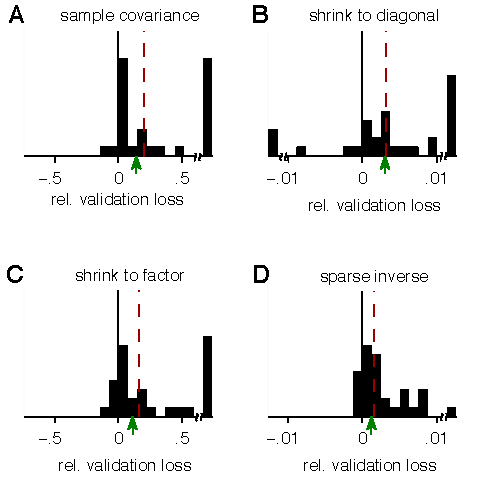
\includegraphics{./figures/Figure04.pdf}}
\end{figure}

\paragraph{Correlation structure and circuit architecture}
Having demonstrated that $C_{\sf sparse+latent}$ dominated the other estimators, we examined the low-dimensional structure revealed by this estimator for individual imaged sites. By design, the sparse+latent estimator finds the mixture of sparse partial correlations between visible neurons and common fluctuations described as latent units. If this estimate dominates, we can hypothesize that it better describes underlying physiological interactions than other estimators, including the sample covariance. In particular, the sparse component of the partial correlation matrix suggests direct interactions between pairs of neurons, whereas the low-rank component suggest common fluctuations such as those caused by common inputs or other collective synchronized activity. 

We examined the structure of the sparse+latent estimate at individual sites (an example site is depicted in Fig.\;\ref{fig:03}). At these sites the regularized estimate of the correlation matrix appeared very similar to the unregularized sample correlation matrix (\figref{05}{A and D}). However, the corresponding partial correlation matrices differed dramatically (\figref{05}{B and E}). The partial correlation was decomposed into sparse and low-rank components (\figref{05}{C}). Although correlations were mostly positive, the sparse partial correlations (or \sq{interactions}), had a much larger fraction of negative values than sample correlations. The sparse component had 82.1\% sparsity (or, conversely, 17.9\% connectivity), which corresponded to the average node degree (interactions per cell) of 52.5 (\figref{05}{G}). The low-rank component had rank 17.

\begin{FPfigure}
    \begin{center}
        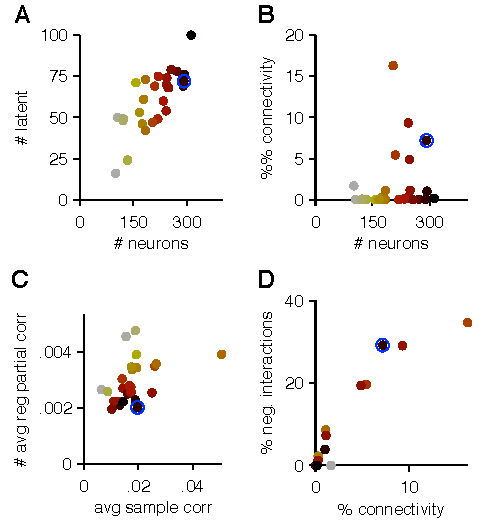
\includegraphics[width=17.35cm]{./figures/Figure05.pdf}
    \end{center}
    \caption{{\bf Example of low-dimensional correlation structure revealed by the sparse+low-rank estimator.}
    {\bf A.} The regularized estimate of the correlation matrix (top-right) closely approximates the sample correlation matrix (bottom left). 
    This close approximation is  also demonstrated by the scatter plot of the correlation coefficients produced by the two estimates ({\bf D}). 
    However, the partial correlation matrices from the two estimate show more pronounced differences ({\bf B} and {\bf E}). 
    {\bf C.} Furthermore, the partial correlation matrix of the regularized estimate is decomposed into a sparse component with 82.2\% off-diagonal zeros (bottom-left) and low-rank component of rank 15 (top-right).
    {\bf F.} The sparse component of the regularized partial correlation matrix had little resemblance to the sample correlations. The gray interval indicates the range of correlations containing 82.2\% of cells pairs, equal to the fraction of zeros in the sparse partial correlation matrix. This interval contained 58.9\% of the partial correlations. 
    {\bf G.} The graphical depiction of the positive (green) and negative (magenta) partial correlations as edges between observed neurons. The line density is proportional to the magnitude of the correlation.
    {\bf H.} A subset of neurons from the center of the cluster shown in {\bf G} showing the regularized partial correlations.
    {\bf I.} The same subset with sample correlations thresholded to match the sparsity of the regularized interactions.
}
\label{fig:05}
\end{FPfigure}

In previous studies of the structure of correlations, a sparse network was produced by thresholding the correlations coefficients at a level deemed significant. A network was formed by connecting neurons whose total correlations exceed this threshold \cite{Golshani:2009,Malmersjo:2013}. There was fairly little overlap between the network of interactions revealed by such thresholding and those revealed by the sparse+latent estimator (\figref{05}{F}). When thresholded to the same sparsity (82.1\%), only 42\% of cell pairs connected in one network were connected in the other while the average magnitude of such correlations was much lower in the case of the regularized estimator (\figref{05}{F, H, and I}). In particular, many low sample correlations translated into negative interactions in the regularized estimate. Indeed, the absence of correlations between pairs of cells that both correlate similarly to several of their neighbors should be considered as significant as a high correlation coefficient. Regularized partial correlations reveal such phenomena whereas regular sample correlations cannot.

The average partial correlations revealed by the sparse+latent estimator at all 31 sites were about 5 times lower than the sample correlations and  less variable across sites (\figref{06}{A}). The average node degree of the sparse component of the partial correlations and the number of inferred latent units varied widely between sites but generally increased with recorded population size (\figref{06}{B and C}). However, there was an inverse relationship between the number of latent units and the average node degree (\figref{06}{D}). Several sites, even with relatively large population sizes, had fairly few pairwise interactions and were dominated by latent units.  These differences have multiple explanations, including differences in brain states and recording quality (neuropil contamination, motion). 

\begin{figure}[!ht]
    \begin{center}
        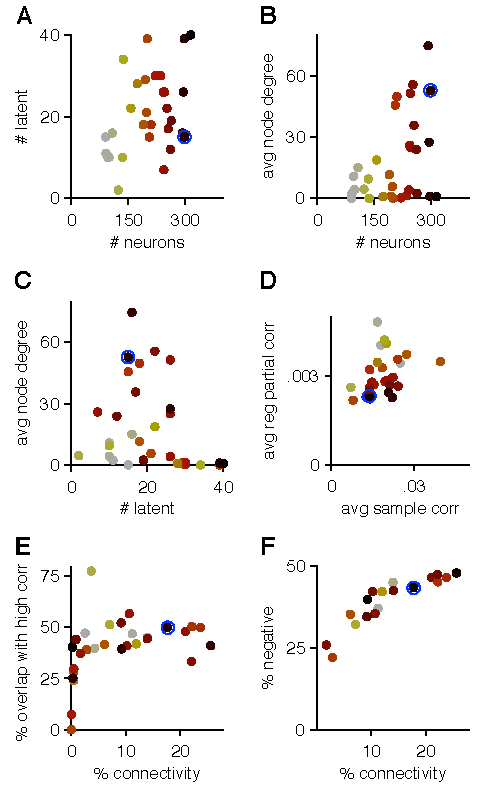
\includegraphics{./figures/Figure06.pdf}
    \end{center}
    \caption{{\bf Properties of sparse+low-rank regularized estimates from all imaged sites}
\\
    {\bf A.} The average sample correlations vs.~average partial correlations for each imaged site. In each plot, the red asterisk indicates the site shown in figures \ref{fig:03} and \ref{fig:05}.
    {\bf B.} The average node degree for sparse partial correlations vs.~population size in each imaged site. 
    {\bf C.} The number of inferred latent units vs.~population size in each imaged site.
    {\bf D.} The number latent units vs.~average node degree for sparse partial correlations for each site.
}
\label{fig:06}
\end{figure}

We also examined the relationship of differences in orientation preference and physical distances (lateral and by depth) between pairs of cells to the average sample correlations, average regularized partial correlations, and inferred connectivity between them (Fig.\;\ref{fig:07}). The average partial correlations fell more rapidly with difference in preferred orientation (\figref{07}{A and D}) and lateral displacements at equal depths ($\pm 25\;\mu$m) (\figref{07}{B and E}), and differences in depth at small ($\pm 25\;\mu$m) lateral displacements (\figref{07}{C and F}).

\begin{figure}[!ht]
    \begin{center}
        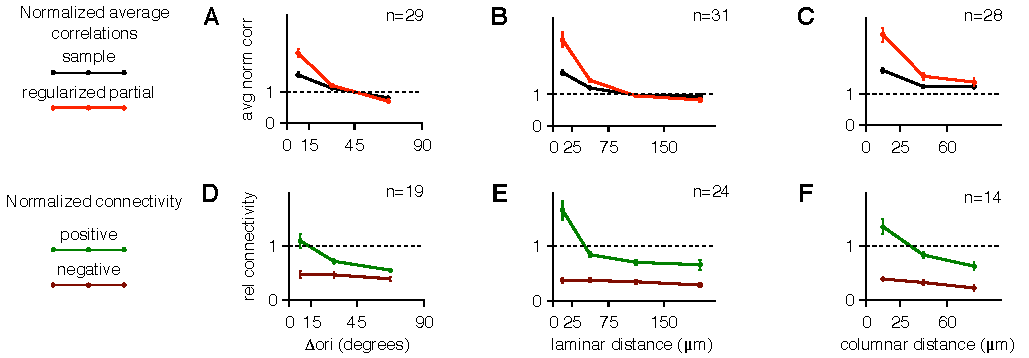
\includegraphics{./figures/Figure07.pdf}
    \end{center}
    \caption{{\bf Dependence of correlations and partial correlations on orientation tuning differences and physical distance between cell pairs.}
    {\bf A--C.} Average partial correlations (red) estimated by $C_{\sf sparse+latent}$ and average sample correlations (black) averaged across multiple imaged sites. In each site, the correlations were normalized by the respective average correlation shown in Fig.\;\ref{fig:06}\,A.  The number $n$ of sites that qualified to be included in the analysis is indicated. Sites were included if they had at least 20 pairs of neurons in each of the intervals. The error bars indicate the standard error of the mean for based on $n$.
    {\bf A.} Average correlations between pairs of neurons tuned to orientation with differences in preferred orientation in the intervals of 0--15$^\circ$, 15--45$^\circ$ and 45--90$^\circ$. 
    {\bf B.} Average correlations between pairs of neurons located at the same depth ($\pm$25$\mu$m) separated by lateral distances in the intervals of 0--25 $\mu$m, 25--75 $\mu$m, 75--150 $\mu$m, and 150+ $\mu$m.
    {\bf C.} Average correlations between pairs of neurons displaced laterally by less than 25 $\mu$m separated in depth by distances in the intervals of 0-25 $\mu$m, 25--60 $\mu$m, and 60+ $\mu$m.
    {\bf D--F.} Normalized connectivity of positive (green) and negative (dark red) interactions from the sparse component obtained from $C_{\sf sparse+latent}$. Normalized connectivity was computed as the fraction of pairs connected by interactions of corresponding signs in each interval divided by the fraction of non-zero interactions across the entire site. Site were included in the analysis only if they had at least 20 cell pairs in each interval. The error bars indicate the standard error of the mean based on the number $n$ of sites included in the analysis.
}
\label{fig:07}
\end{figure}

The connectivity expressed by the partial correlations in the regularized estimate had different organization for positive and negative interactions. Positive interactions fell rapidly as a function of difference in preferred orientation (\figref{07}{D}), lateral displacements (\figref{07}{E}), and displacement in depth (\figref{07}{F}). Negative interactions were much less selective (\figref{07}{D--F}).

\section*{Discussion}
\paragraph{Functional connectivity}
Effective phenomenological or statistical descriptions of neural activity can serve as a starting point for investigation of underlying physiological mechanisms.  For example, the discoveries of receptive fields and tuning properties of single neurons, over the past 60 years, have led to fruitful hypotheses about the underlying patterns of synaptic connectivity and principles of neural coding, and to the discovery of other organizational principles such as various cortical feature maps \cite{Reid:2012}.  The search for similarly effective descriptions of observed \emph{multineuronal} activity patterns that are not reducible to the response properties of the individual cells has produced various statistical expressions collectively known as \sq{functional connectivity}.  Functional connectivity is commonly expressed as the degree of correlation, synchronization, or other forms of statistical association between neurons and is thought to reflect internal local recurrent connectivity, shared interactions with other regions, or endogenous network activity.  To remove the confounding effects of stimuli, the average stimulus responses are usually subtracted or otherwise accounted for. Although various measures of functional connectivity are only phenomenological descriptions of population activity, they provide experimental neuroscientists with tools to relate population activity to the anatomical and functional architecture of neural circuits and to generate hypotheses about underlying mechanisms. 

\paragraph{Functional connectivity as a network of pairwise interactions}
The intended purpose of many studies of functional connectivity is to estimate the circuit�s anatomical connectivity solely from the observed multineuronal spiking activity.  For example, characteristic peaks and troughs in the pairwise cross-correlograms of recorded spike trains contain statistical signatures of directional monosynaptic connections or shared synaptic inputs \cite{Gerstein:1964, Perkel:1967, Moore:1970, Alonso:1998, Denman:2013}.  Such signatures are still ambiguous as they can arise from diverse network effects other than direct synaptic connections \cite{Aertsen:1989}.  With simultaneous recordings from a larger subset of neurons in the circuit, ambiguities can be resolved by inferring the conditional dependencies between pairs of neurons.  Since direct causal interactions between neurons produce statistical dependency even after conditioning on the state of the rest of the network, conditionally independent neurons can be inferred to lack a direct causal influence.  Such conditional dependencies can be inferred by fitting a probabilistic model of the joint population activity. For example, generalized linear models (GLMs) have been constructed to include biophysically plausible synaptic integration and membrane kinetics, individual neurons� stimulus drive, and a network of synaptic couplings \cite{Pillow:2008}.  Another family of models are maximum entropy models that are constrained by the observed pairwise correlations \cite{Schneidman:2006, Tkacik:2006, Yu:2008, Tang:2009, Shlens:2009} .  Although not informed by physiology, maximum entropy models are attractive because they account for the observed statistics with fewest other assumptions about the distribution: the investigator need only choose which statistics to match.  Under the multivariate normal distribution, the conditional dependencies between pairs of neurons are expressed by the partial correlations between them.   Each probabilistic model, fitted to the same data may reveal a different network of \sq{interactions},  \emph{i.e.}\;conditional dependencies between pairs of neurons. 

The inference of the conditional dependencies also depends on the completeness of the recorded population:  To properly condition the interaction between a pair of neurons on the activity of the other neurons under a given probabilistic model, the recording must include all the other neurons with which the pair can potentially interact. Otherwise, interactions with the unobserved portions of the circuit will introduce false conditional dependencies between the observed neurons. For this reason, the most successful applications of statistical models of population activity thus far have been in in vitro preparations of the retina or cell cultures where high-quality recordings from the complete populations have been possible \cite{Pillow:2008}. When inserted in cortical tissue, electrode arrays record from a small fraction of cells in a given volume, limiting the validity of the inference of the conditional dependencies between pairs of cells. Perhaps for this reason, until our study, partial correlations have not been used to describe the functional connectivity between cortical neurons.  Despite this limitation, many studies have fitted probabilistic models to multielectrode recordings and analyzed the structure of the resulting conditional dependencies \cite{Tang:2008, Yu:2008}.  

Because the validity of the inference of interactions from probabilistic models depends on both the correctness of their mathematical form in the model and the completeness of the recorded population, it is far from clear which approach provides best correspondence to the anatomical connectivity in the circuit, with no experimental evidence yet available to address this question.  The result is often treated as a graphical representation of the functional connectivity without a statement about its anatomical implications.  Whatever these implications may be, investigators have applied graph-theoretical analyses to the inferred networks to make statements about the design principles and efficiency of circuit architectures \cite{Feldt:2011, Yu:2008, Malmersjo:2013}. 

Two-photon imaging of population calcium signals presents unique advantages for the estimation of functional connectivity despite some of the disadvantages.  The temporal resolution of calcium signals is limited by calcium dye kinetics. Fast imaging techniques combined with advanced spike inference algorithms have been demonstrated to provide millisecond-scale temporal resolution of single action potentials \cite{Grewe:2010, Katona:2012, Cotton:2013}. However, such high temporal precision comes at the cost of the accuracy of the inferred spike rates: better accuracy can be achieved when calcium signals are analyzed on the temporal scales of tens of milliseconds \cite{Cotton:2013}.  For what calcium imaging lack in temporal resolution, it make up in spatial resolution and the ability to characterize the spatial arrangements of cells and identify their types.  Recently, advanced imaging techniques have allowed recording from nearly every cell in a volume of cortical tissue in vivo \emph{in vivo} \cite{Katona:2012, Cotton:2013} and even from entire nervous systems \cite{Leung:2013, Ahrens:2013}.  Such completeness may open new opportunities for inferring networks of conditional dependencies between neurons with greater validity than with electrophysiological recordings.  

The low temporal resolution of calcium signals limits the use of functional connectivity methods that rely on millisecond-scale binning of signals (cross-correlograms, some GLMs, and maximum entropy models on the binary domain).  Most studies of functional connectivity have relied on instantaneous sample correlations \cite{Greenberg:2008, Golshani:2009, Hofer:2011, Malmersjo:2013} .  Although some investigators have interpreted such correlations as indicators of (chemical or electrical) synaptic connectivity, most used them as more general indicators of functional connectivity without a statement about underlying mechanisms. 

In our study, we sought to express pairwise connectivity networks among neurons in local cortical microcircuits. We hypothesized that partial correlations would correspond more closely to underlying mechanisms than sample correlations.  Since neurons form synaptic connections mostly locally and sparsely \cite{Perin:2011}, we a priori favored solutions in with sparse partial correlations.  The importance of partial correlations may be justified by the principle of maximum entropy: The maximum entropy distribution on discrete or continuous multivariate domains constrained by the observed mean firing rates, their variances, and correlations is the multivariate normal distribution.  The interactions (conditional dependencies) between pairs of neurons inferred by this distributed are expressed by the precision matrix (inverse of the covariance) or, equivalently, by the matrix of the pairwise partial correlations. Therefore, under the aforementioned assumptions that the recorded population is sufficiently complete and that the model correctly represents the nature of interactions, the network of partial correlations can be hypothesized to be a better representation of functional dependencies than sample correlations.

\paragraph{Functional connectivity as coactivations}
Another approach to describe the functional connectivity of a circuit is to isolate patterns of multineuronal coactivations \cite{Gerstein:1989, Chapin:1999, Peyrache:2010, Ch:2010, Lopes:2011, Lopes:2013}. Depending on the method of their extraction, coactivation patterns may be referred to as \emph{assemblies}, \emph{factor loadings}, \emph{principal components}, \emph{independent components}, \emph{activity modes}, \emph{eigenvectors}, or \emph{coactivation maps}. Coactivation patterns could be interpreted as signatures of Hebbian cell assemblies \cite{Gerstein:1989, Ch:2010}, \emph{i.e.}\;groups of tightly interconnected groups of cells involved in a common computation.  Coactivation patterns could also be explained as shared input from unobserved parts of the circuit.  Coactivations could also be explained by global network fluctuations modulating the activity of the local circuit \cite{Okun:2012}.

Coactivation patterns and pairwise connectivity are not mutually exclusive since assemblies arise from patterns of synaptic connectivity, but analysis of coactivations method shifts the focus from detailed interactions to the collective behavior.  

In our study, the analysis of functional connectivity through modes of coactivations was represented by the factor analysis estimator $C_{\sf factor}$.  

\paragraph{Combining pairwise interactions and coactivations}
In the effort to account for the joint activity patterns that are poorly explained by pairwise interactions, investigators have augmented models of pairwise interactions with additional mechanisms such as latent variables \cite{Koster:2013},  high-order correlations \cite{Ganmor:2011}, or global network fluctuations \cite{Tkacik:2013}.

In our study, we combined pairwise interactions with collective coactivations by applying the recently developed numerical techniques for the inference of the partial correlation structure in systems with latent variables \cite{Chandrasekaran:2010, Ma:2013}.  The resulting estimator, $C_{\sf sparse+latent}$, effectively decomposed the functional connectivity into a sparse network of pairwise interactions and coactivation mode vectors.
\paragraph{Addressing ill-posedness}
Inferring the conditional dependencies between variables in a probabilistic model is an ill-posed problem: small variations in the data produce large errors in the inferred network of dependencies.  The problem becomes increasingly worse as the size of the recorded population of neurons increases until such models lose their statistical validity \cite{Roudi:2009}.  As the recorded neuronal population sizes increased gradually, experimental neuroscientists addressed this problem by extending the recording durations to keep sampling noise in check and verified that existing models are not overfitted and that the stationarity assumption are observed\cite{Tkacik:2013}.  However, with ambitious projects, such as the BRAIN initiative currently underway \cite{Alivisatos:2013} aiming to record from significantly larger populations, the problem must be addressed by regularizing the solution. Regularization limits the solution to a smaller subspace to counteract the effect of the sampling noise in the empirical data. However, limiting the solution to an inappropriate subspace does not allow significant improvement. 

Several strategies have been developed to limit the model space in order to improve the quality of the estimate. For example, \cite{Ganmor:2011} developed a heuristic rule to identify the most significant features that must be fitted by a maximum entropy model for improved performance in retina. Generalized linear models typically employ $L_1$ penalty terms to constrain the solution space and to effectively reduce the dimensionality of the solution \cite{Pillow:2008}.  

In our study, regularization was also accomplished by dimensionality reduction (feature selection) schemes to produce sparse, constrained solutions.

Since optimal regularization schemes are specific to systems under investigation, the inference of functional connectivity in big neural data will entail the search for optimal regularizations that may involve combinations of heuristic rules and numerical techniques specifically designed for each type of neural circuit.

\paragraph{Model selection}
In our study, the covariance matrix estimators were evaluated with respect to the cross-validated normal log likelihood.  However, this does not limit the applicability of its conclusions to normal distributions. Indeed the major findings in this paper could be reproduced with respect to other loss functions (compare Fig.~\ref{fig:04} and Fig.~S\ref{supp:02}).  Other probabilistic models, fitted to the same data, would also serve as estimators of the covariance matrix.  If a different model yields better estimation of the covariance matrix than the estimator proposed here, we believe that its structure should deserve consideration as the better representation of the functional connectivity.

The results of model selection must be interpreted with caution.  As we demonstrated by simulation, a simple model can produce a better estimate even if it does not correctly represent the real dependencies in the data than a more complex model with correct representation of dependencies.   Therefore, showing that a more constrained model has better cross-validated performance than a more complex model does not support the inference that it reveals a better representation of dependencies in the data.  This caveat is related to the phenomenon known as \emph{Stein�s Paradox} \cite{Efron:1977}: in which the biasing of an estimate toward an arbitrary target is guaranteed to produce \emph{some} improvement. 

\paragraph{Physiological interpretation and future directions}
Although the network of interactions inferred by the optimal estimator, $C_{\sf sparse+latent}$, alludes synaptic interactions, it is unlikely that the anatomical and functional networks are identical.  The improved estimation performance gives the model extra credence over other estimates of the functional connectivity.  The inferred interaction network was substantially different from that inferred from by considering the network of most significant sample correlations (\figref{05}{F, H, and I}).  In particular, sample correlations do not draw attention to the absence of correlation between a pair of neurons that should be strongly correlated based on their common correlations with other neurons.  The $C_{\sf sparse+latent}$ estimator identified many such pairs and inferred negative interactions between them (\figref{05}{F}).  The resulting network had a larger fraction of negative interactions than the fraction of negative correlations in the sample correlation matrix.  The negative interactions had a distinct spatial organization from   Reproducing our study with labeled interneurons of various types could indicate whether the negative interactions 

The estimator effectively decomposed the correlation structure into two distinct components: pairwise interactions and common coactivation modes denoted as \sq{latent units}.   Since the distinction led to improved estimation, the two types of components could be further investigated.  For example, slow-wave network fluctuations due to anesthesia or slow-wave sleep could be strongly reflected on the common components/latent units but much less on the pairwise interactions. Previous studied found that correlations measured under anesthesia retained little in common to correlations measured in wakefulness and concluded that studies of the anesthetized brain did not inform about its behaviorally relevant functions \cite{Greenberg:2008}.  When conditioned on the brain state, optimal estimation of covariance matrices in dense cortical networks could reveal that slow-wave activity alters the common components but does not affect the pairwise interactions as strongly.  The correlation structure also changes as a function of the stimulus condition \cite{Cotton:2013} on time scales that are much faster than changes in the anatomical connectivity. Descriptions of specific changes in the functional connectivity due to stimulus properties could shed light on how circuits orchestrate their activity to represent diverse stimuli.

The malleability of the joint structure of activity in populations of neurons makes functional connectivity statistics indispensible wholly apart from the ability to infer the anatomical connectivity.  Effective statistical descriptions of the functional connectivity will need to be developed to infer the most significant features of the functional organization in large ensembles of neurons from limited data.  These approaches will need to rely on techniques exemplified by our study: selection among multiple mathematical representations of dependencies, regularization, and model selection. 
 
\section*{Methods}
% You may title this section "Methods" or "Models". 
% "Models" is not a valid title for PLoS ONE authors. However, PLoS ONE
% authors may use "Analysis" 
\paragraph{Surgery and two-photon Imaging}
All procedures were conducted in accordance with the ethical guidelines of the National Institutes of Health and were approved by the Baylor College of Medicine IACUC.  The surgical procedures and data acquisition were performed as descrbed in \cite{Cotton:2013}. Briefly, C57BL/6J mice (aged p40--60) were used. Anesthesia was initiated with isoflurane (3\%) and the mixture of fentanyl (0.05 mg/kg), midazolam (5 mg/kg), and medetomidine (0.5 mg/kg), with boosts of half the initial dose every 3 hours.  A craniotomy was performed over the right primary visual area.  Membrane-permeant calcium indicator Oregon Green 488 BAPTA-1 AM (OGB-1, Invitrogen) was loaded by bolus injection.  The craniotomy was sealed using a glass coverslip secured with dental cement. 

Calcium imaging began 1 hour after dye injection.  All imaging was performed using the 3D-RAMP two-photon microscope described in \cite{Cotton:2013}. First, A 3D stack was acquired and cells manually segmented.  To collect calcium signals, the system repeated hopped between the selected neurons. 
\paragraph{Visual stimulus}
Full-field drifting gratings with 90\% contrast, luminance of 10 cd/m$^2$, spatial frequency of 0.08 cycles/degree, and temporal frequency of 2 cycles/s. Two sets of stimuli were presented for each imaging site: the first to map directional tuning and the second to estimate noise correlations. Directional tuning was map using a pseudo-random sequence of drifting gratings at sixteen equally spaced directional of motion changing at 2 Hz for 3 min without blanks. The data for covariance estimation were collected during presentations of full-field drifting gratings with the same parameters as those used in directional tuning except only two directions (in 9 dataset) or five directions (in 22 datasets) were used and the presentations lasted 1 second and, separated by 1-second blanks.  Each stimulus condition was presented at least 180 times. 
\paragraph{Data processing}
All data were processed in MATLAB using the DataJoint data processing chain toolbox ({\tt datajoint.github.com}) first developed in our lab. 

The collected fluorescent traces were deconvolved to reconstruct the firing rates for each neuron. First, the first principal component was subtracted from the traces, which reduced common mode noise related to small movement and cardiovascular artifacts. The resulting traces were low-pass filtered below 0.1 Hz and downsampled to 20 Hz. Firing rates were estimated using a fast non-negative deconvolution algorithm \cite{Vogelstein:2010}.

Orientation tuning was computed by fitting the mean firing rates in response to gratings of directions $\phi$ with two-peaked von Mises tuning functions of the form $f(\phi)=a + b\exp\left[\frac 1 w(\cos(\phi-\theta)-1) \right] + c\exp\left[\frac 1 w(\cos(\phi-\theta+\pi)-1) \right]$ where $b\ge c$ are amplitudes of the two respective peaks, $w$ is the tuning width, and  $\theta$ is the preferred direction. The significance of the fit was determined by the permutation test: the labels of the direction were randomly permuted 10,000 times.  The $p$-value of the fit was computed as the fraction of permuted datasets for which the $R^2$ value of the tuning function fit exceeded that of the real data.  Cells were considered tuned for $p$-values not exceeding $0.05$.

For covariance estimation, the analysis was limited to the period with 2 or 5 stimulus conditions and lasted between 12 and 20 mins.  Only traces whose average deconvolved signal was greater than 1\% of the median of the recorded population were included in the analysis.  
\paragraph{Cross-validation}
To compare the performance of the estimator against each other, we used conventional 10-fold cross validation to measure cross-validation loss (Eq.~\ref{eq:cv-loss}). Briefly, each recording was split into 30 blocks of equal duration.  The 30 blocks were then grouped randomly into 10 datasets with 3 blocks in each.  This procedure ensured sufficient independence between the 10 datasets while still ensuring that each dataset included data from different parts of the recording.   Then, each dataset was used as the testing dataset with the rest of the data used for estimating the covariance matrix.  

Since each of the regularized estimators had one or two hyperparameters, we used \emph{nested cross-validation}.  The outer loop evaluated the performance of the estimators with optimal values of the hyperparameters.  The optimization of the hyperparameters was performed within the inner loop in two phases: random search to find a good starting point and pattern search to find the global minimum.  The inner cross-validation loop subdivided the training dataset from the outer loop to perform 10-fold cross-validation in order to evaluate each choice of the hyperparameter values.  Thus the size of the training dataset within the inner loop comprised 81\% of the entire recording.

When cross-validation loss was not required, only the inner loop of cross-validation was used, applied to the entire dataset.  This approach was used to compute the covariance matrix estimates and their excess-loss in the simulation study (\figref{02}{\;rows 3 and 4}) and to analyze the partial correlation structure of the sparse+latent estimator (Fig.~\ref{fig:05}--\ref{fig:07}).
\paragraph{Covariance Estimation}
Within the inner loop of cross-validation, covariance matrix estimation was performed with fixed hyperparameter values provided by the search algorithm.  The computation of each regularized estimator only required the sample covariance matrix $C_{\sf 0}$ of the training dataset. 

Estimator $C_{\sf diag}$ (Eq.~\ref{eq:c-diag})  used two hyperparameters: the covariance shrinkage intensity $\lambda \in [0,1]$ and variance shrinkage intensity $\alpha \in [0,1]$.  The variances (the diagonal of $C_{\sf 0}$) were shrunk toward (linearly mixed with) their mean value:
\begin{equation}
D = (1-\alpha)C_{\sf 0}\circ I + \alpha \frac 1 p \Tr(C_{\sf 0}) I
\end{equation}
Then the diagonal matrix $D$ was used as the target of covariance shrinkage (Eq.~\ref{eq:c-diag}) to produce the final regularized estimate.

The {\tt corpcor} package in the programming language R also implements this estimator \cite{Schafer:2010}, although its analytical optimization of the shrinkage intensities is based on the mean squared error whereas we optimized them with respect to the loss function in Eq.~\ref{eq:loss}.

Estimator $C_{\sf factor}$ used two hyperparameters: the number of latent factors $d$ and the shrinkage intensity $\lambda \in [0, 1]$.  
The $p\times d$ factor loading matrix $L$ and individual variances $\Psi$ were computed by solving the minimization problem
\begin{equation}
(L,\Psi) = \argmin\limits_{\tilde L,\tilde\Psi} \loss{\tilde L + \tilde\Psi,C_{\sf 0}},
\end{equation}
which we solved by an expectation-maximization (EM) algorithm.  Under our chosen loss function (Eq.~\ref{eq:loss}), this is equivalent to maximum likelihood estimation of $L$ and $\Psi$ under the multivariate Gaussian distribution.  The final regularized estimate is obtained by linear shrinkage toward the factor model (Eq.~\ref{eq:c-factor}). 

Estimator $C_{\sf sparse}$  has one hyperparameter $\lambda$, which regulates the sparsity of its precision matrix $S$. The precision matrix is computed in two steps: First, the zero structure $Z$ is determined by minimizing the $L_1$-penalized loss.
\begin{equation}
Z = \argmin\limits_{\tilde Z \succ 0} \loss{{\tilde Z}^{-1},C_{\sf 0}} + \lambda \|\tilde Z \|_1
\end{equation}
where $\tilde Z\succ 0$ denotes the constraint that $\tilde Z$ be a positive definite matrix and $\|\tilde Z\|_1$ is the element-wise $L_1$ norm of the matrix $\tilde Z$. This problem formulation is known as \emph{graphical lasso} \cite{Friedman:2008}. To solve this minimization problem, we modified the alternative-direction method of multipliers (ADMM) algorithm developed by \cite{Ma:2013}. 
Then, after the zero structure was determined, the remaining coefficients were fitted without penalty:
\begin{equation}
S = \argmin\limits_{\tilde S \in Z^\sharp} \loss{\tilde S,C_{\sf 0}},
\end{equation}
where $Z^\sharp$ denotes the set of positive-definite matrices with zeros in all entries where entries of $Z$ equal zero.  This step was also solved by ADMM.  Then the final estimate is the inverse of $S$ (Eq.~\ref{eq:c-sparse}). Unlike $C_{\sf diag}$ and $C_{\sf factor}$, this estimator does not include linear shrinkage: the selection of the sparsity level provides sufficient flexibility to fine tune the regularization level.

Estimator $C_{\sf sparse+latent}$ has two hyperparameters: the number of latent units $d$ and the sparsity level $\lambda$. It estimates the larger sparse precision matrix $S^\ast$ of the joint distribution of the $p$ observed neurons and $d$ latent units.  
\begin{equation}
S^\ast=
\begin{pmatrix}
S & S_{12} \\
S_{12}^\T & S_{22}
\end{pmatrix},
\end{equation}
where the $p\times p$ partition $S$ corresponds to the visible units and expresses their partial correlation structure, and $S_{12}$ and $S_{22}$ are of size $p\times d$ and $d\times d$, respectively.
Then the covariance matrix of the observed population is 
\begin{equation}
C_{\sf sparse+latent} = (S^\ast)^{-1} = \left(S-S_{12}S_{22}^{-1}S_{12}^\T\right)^{-1}
\end{equation}
The matrix $ S_{12}S_{22}^{-1}S_{12}^\T$ has rank $d$. Rather than searching for the optimal sparse structure of $S_{12}$ and $S_{22}$, an ill-posed problem, we estimated these components together as one positive-definite $p\times p$ matrix $L$ of rank $d$.

The estimate is found in two steps. First, we use the ADMM algorithm to find the zero structure of $S$ by minimizing the $L_1$-penalized loss \cite{Chandrasekaran:2010,Ma:2013}:
\begin{equation}
(Z,\cdot) = \argmin\limits_{\tilde Z,\tilde L} \loss{\tilde Z-\tilde L} + \|\tilde Z\|_1
\end{equation}
Then we find the sparse and low-rank components of the precision matrix by minimizing the loss 
\begin{equation}
(S,L) = \argmin\limits_{\tilde S \in Z^\sharp,\tilde L} \loss{\tilde S-\tilde L }
\end{equation}

The partial correlation matrix computed from the overall estimate, computed from $C_{\sf sparse+latent}$ according to Eq.~\ref{eq:partial}, includes the effects of interactions between the visible and latent units.  This estimate of the partial correlations was used in analyses where sparsity was not required (\figref{05}{B and E} and \figref{06}{A}, and \figref{07}{A--C}).  For analyses that required a sparse network (\figref{05}{F, G, H} and \figref{06}{B, D} and \figref{07}{D--F}) was computed using the extended precision matrix $S^\ast$:
\begin{equation}
P_{\sf sparse} = (S\circ I)^{-\frac 1 2} S  (S\circ I)^{-\frac 1 2}
\end{equation}

The MATLAB code for these computations is available at {\tt http://github.com/atlab/cov-est}.


\paragraph{Simulation}
For simulation, ground truth covariance matrices were produced by taking 150 independent samples from an artificial population of 50 independent, identically normally distributed units. The covariance matrices were then subjected to the respective regularizations to produce the ground truth matrices for the simulation studies (\figref{02}{\,row 2}. Samples were then generated by multivariate normal distributions with the respective true covariance matrices and estimated by each of the estimators. 

\section*{Acknowledgments}
We thank Genevera Allen for a helpful discussion.  We thank Eftychios Pnevmatikakis for helpful suggestions and feedback.

% The bibtex filename
\bibliography{references.bib}


%\section*{Figure Legends}
\newpage
\section*{Supporting Information}
\setcounter{figure}{0}

\begin{figure}[!ht]
\begin{center}
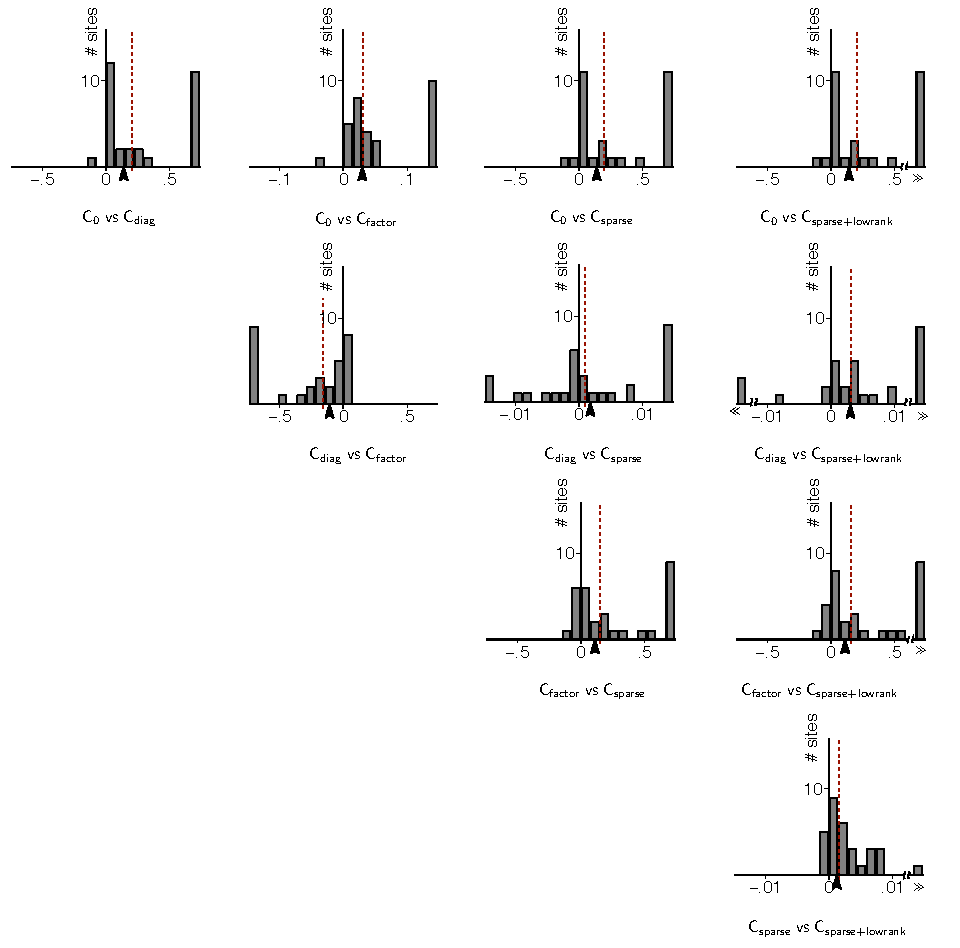
\includegraphics{./figures/Figure-Supp01.pdf}
\end{center}
\caption{{\bf All-to-all performance comparisons of the sample covariance matrix and the four regularized estimators with respect to multivariate normal cross-validation loss.}
}
\label{supp:01}
\end{figure}


\begin{figure}[!ht]
\floatbox[{\capbeside\thisfloatsetup{capbesideposition={right,center},capbesidewidth=8.3cm}}]{figure}[\FBwidth]
{\caption{{\bf The sparse+latent estimator outperforms the other estimators with respect to quadratic cross-validation loss $\loss{C,C_{\sf 0}^\prime}=\frac 1 {p^2}\Tr(C^{-1}C_{\sf 0}^\prime-I)^2$.}
}
\label{supp:02}}
{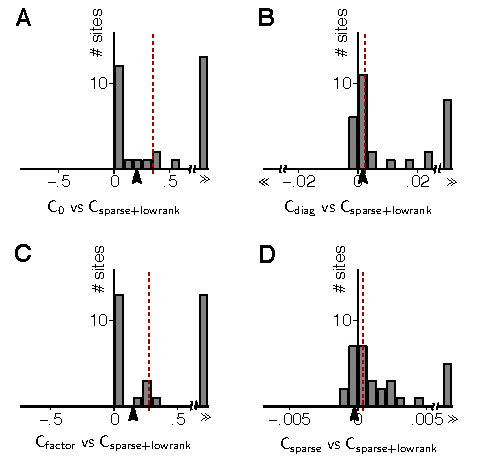
\includegraphics{./figures/Figure-Supp02.pdf}}
\end{figure}


\end{document}
